\documentclass[10pt]{beamer}

\usetheme{metropolis}
\usepackage{appendixnumberbeamer}

\usepackage{booktabs}
\usepackage[scale=2]{ccicons}
\usepackage{graphicx}
\usepackage{hyperref}
\usepackage{circuitikz}
\usepackage{pdflscape}
\usepackage{smartdiagram}

\usepackage{color}
\usepackage{listings}

\lstset{
	basicstyle=\footnotesize\ttfamily,
    keepspaces=true,
    showstringspaces=false,
    language=PHP,
    commentstyle=\ttfamily,
}

\usepackage[OT4]{polski}
\usepackage[utf8]{inputenc}

\usepackage{pgfplots}
\usepgfplotslibrary{dateplot}

\usepackage{xspace}
\newcommand{\themename}{\textbf{\textsc{metropolis}}\xspace}

\setbeamertemplate{frame footer}{}
\setbeamertemplate{frame numbering}{}

\usetikzlibrary{shapes,arrows}

\tikzstyle{decision} = [diamond, draw, fill=blue!20, 
    text width=4.5em, text badly centered, node distance=3cm, inner sep=0pt]
\tikzstyle{block} = [rectangle, draw, fill=blue!20, 
    text width=5em, text centered, rounded corners, minimum height=4em]
\tikzstyle{line} = [draw, -latex']
\tikzstyle{cloud} = [draw, ellipse,fill=red!20, node distance=3cm,
    minimum height=2em]


\title{Uwierzytelnianie i autoryzacja użytkowników}

\subtitle{Projektowanie i programowanie systemów internetowych I}
\author{mgr inż. Krzysztof Rewak}
\date{\today}
\institute{Wydział Nauk Technicznych i Ekonomicznych \\ Państwowa Wyższa Szkoła Zawodowa im. Witelona w Legnicy}

\begin{document}

\maketitle

\begin{frame}{Plan prezentacji}
  \setbeamertemplate{section in toc}[sections numbered]
  \tableofcontents[hideallsubsections]
\end{frame}


\section{Definicje}

\begin{frame}{Użytkownik}
	Kim jest \textbf{użytkownik}?
\end{frame}

\begin{frame}{Użytkownik}
	Uogólniając będzie to osoba korzystająca z systemu - w tym wypadku, internetowego.
\end{frame}

\begin{frame}{Użytkownik}
	Czyli kto?
	
	\begin{itemize}
		\item gość wchodzący pierwszy raz na naszą witrynę?
		\item osoba znająca hasło dostępu?
		\item osoba z prywatnym zestawem hasła i nazwy użytkownika?
		\item odpytanie przez API?
	\end{itemize}
\end{frame}

\begin{frame}[fragile]{Użytkownik}
	\begin{lstlisting}
public class User {

    private String id;
    private String name;
    private String password;

}
	\end{lstlisting}
	
	Czy to wystarczy do obsługi użytkowników?
\end{frame}

\begin{frame}{Uwierzytelnianie}
	Jeżeli system internetowy udostępnia możliwość tzw. zalogowania się użytkownika, należy wówczas mówić o mechanizmie \textbf{uwierzytelniania}.
\end{frame}

\begin{frame}{Uwierzytelnianie}
	Uwierzytelnianie (ang. \emph{authentication}) (ale nigdy nie \emph{autentykacja}!), czyli weryfikacja użytkownika, najczęściej polega na porównaniu uprzednio zapisanych danych z danymi wpisywanymi przez użytkownika.
\end{frame}

\begin{frame}{Autoryzacja}
	Nigdy nie należy mylić uwierzytelniania z \textbf{autoryzacją}, która jest sprawdzeniem czy dany użytkownik może wykonać daną operację.
\end{frame}

\section{Uwierzytelnianie z sesją}

\begin{frame}{Gdzie spotkać uwierzytelnianie?}
	\begin{figure}[t]
		\centering
		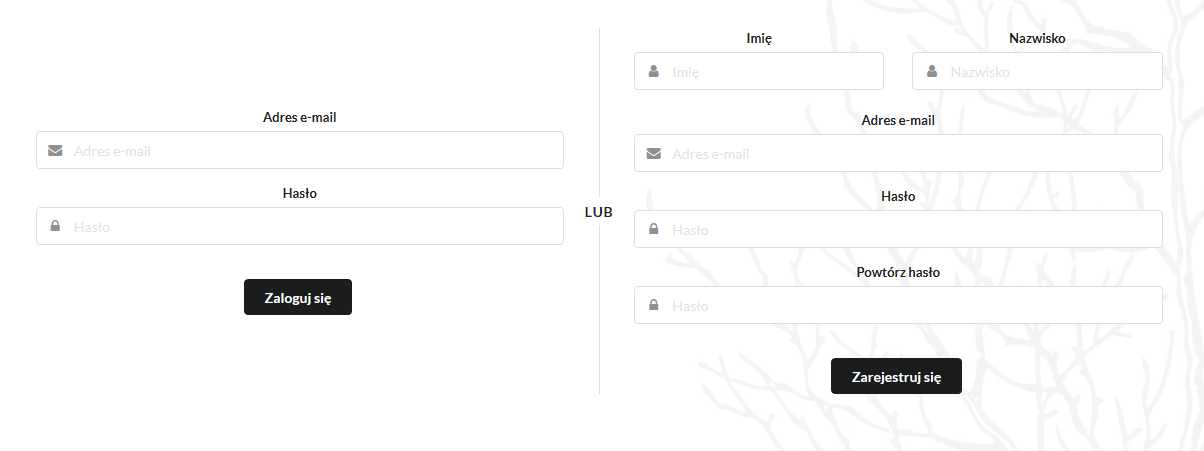
\includegraphics[width=\linewidth]{forms.png}
		\caption{Przykładowy formularz logowania i rejestracji}
	\end{figure}
\end{frame}

\begin{frame}{Gdzie spotkać uwierzytelnianie?}
	\begin{itemize}
		\item poczta elektroniczna
		\item bankowość elektroniczna
		\item portale społecznościowe
		\item aplikacje użytkowe
	\end{itemize}
\end{frame}

\begin{frame}{Gdzie spotkać uwierzytelnianie?}
	\begin{itemize}
		\item praktycznie wszędzie
	\end{itemize}
\end{frame}

\begin{frame}{Czym można uwierzytelniać?}
	W podstawowym wariancie będzie to \textbf{unikalna} nazwa użytkownika lub jego adres poczty elektronicznej oraz prywatne hasło.
	
	Niektóre systemy umożliwiają logowanie się loginem, mejlem lub numerem telefonu. Inne wymagają zapamiętania odgórnie narzuconej nazwy użytkownika. Jaka jest najsensowniejsza forma? To już zależy od upodobań klienta.
\end{frame}

\begin{frame}[fragile]{\emph{Crème de la crème}}
	\begin{lstlisting}
public function loginAction(Request $request): Response {

  $user = $this->findUserByLogin($request->login);

  if($user) {
    if($this->checkHash($request->password, $user->password)) {
      $this->registerSession($user);
      $this->responseArray->setSuccessStatus();

      return $this->renderResponse();
    }
  }

  $this->security->hash(rand());
  return $this->renderResponse();

}
	\end{lstlisting}
\end{frame}

\begin{frame}{Krok po kroku}
	Uwierzytelnianie może wyglądać następująco:
	\begin{enumerate}
		\item użytkownik przesyła swój login i hasło przez formularz
		\item sprawdzane jest czy użytkownik o takim loginie istnieje
		\item jeżeli istnieje, wówczas sprawdzane jest czy przesłane hasło pasuje do tego uprzednio zapisanego
		\item jeżeli pasuje, wówczas użytkownik powinien zostać zalogowany
		\item jeżeli hasło nie pasuje lub login nie istnieje, użytkownik nie powinien zostać zalogowany
	\end{enumerate}
\end{frame}

\begin{frame}{Krok w bok}
	O czym warto pamiętać, nad czym warto się zastanowić, co warto zaimplementować?
	\begin{itemize}
		\item użytkownik musi zostać poinformowany o statusie akcji, ale niekoniecznie o wszystkich jej szczegółach (\emph{podany błędy login lub hasło} zamiast \emph{taki użytkownik w bazie danych nie istnieje})
		\item czy każdy użytkownik może się zalogować? (co ze zbanowanymi lub nieaktywowanymi?)
		\item czy obsługa formularza jest zabezpieczona?
	\end{itemize}
\end{frame}

\begin{frame}{Ale czym tak naprawdę jest logowanie?}
	Do uwierzytelniania wykorzystuje się pojęcie \textbf{sesji}, która jest zapamiętywana na serwerze i najczęściej identyfikowana przez przechowywany w ciasteczku identyfikator.
	
	Sesję można przechowywać w plikach, bazie danych, systemach pamięci podręcznej lub innych formach. Większość nowoczesnych frameworków webowych oferuje wbudowane i gotowe rozwiązania sesji.
\end{frame}

\begin{frame}[fragile]{Więc czym tak naprawdę jest wylogowanie?}
	\begin{lstlisting}
public function logoutAction(): Response {
  $this->session->remove("auth");

  $this->responseArray
    ->setMessage("Wylogowano poprawnie.")
    ->setSuccessStatus();

  return $this->renderResponse();
}
	\end{lstlisting}
\end{frame}

\section{Uwierzytelnianie bez sesji}

\begin{frame}{Bezsesyjność}
	Co się dzieje, jeżeli frontend stoi na jednym serwerze, a backend na drugim?
\end{frame}

\begin{frame}{Bezsesyjność}
	Wówczas obie aplikacji muszą ze sobą rozmawiać w pewien sposób (REST?) poprzez protokół HTTP.
\end{frame}

\begin{frame}{JWT}
	\begin{figure}[t]
		\centering
		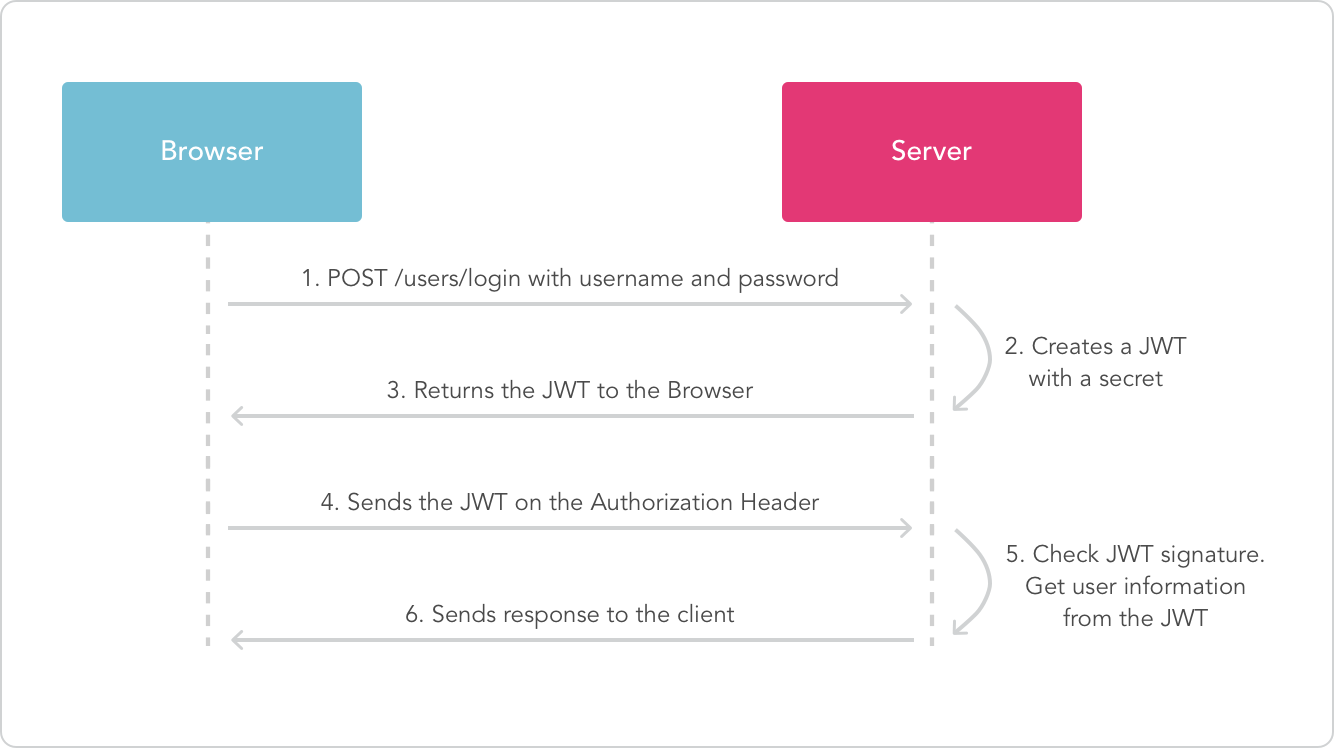
\includegraphics[width=\linewidth]{jwt.png}
		\caption{https://jwt.io/introduction/}
	\end{figure}
\end{frame}

\section{Autoryzacja}

\begin{frame}{Kto i co?}
	Autoryzacja jest mechanizmem, który odpowiada na pytanie \emph{kto co może?}
\end{frame}

\begin{frame}{Kto i co?}
	Najprostszy przykład:
	\begin{itemize}
		\item kto: zalogowany użytkownik ID = 1
		\item co: może wejść do edycji swojego profilu
	\end{itemize}
	
	ale:
	\begin{itemize}
		\item kto: zalogowany użytkownik ID = 1
		\item co: nie może wejść do edycji nieswojego profilu
	\end{itemize}
	
	oraz:
	\begin{itemize}
		\item kto: niezalogowany użytkownik
		\item co: nie może wejść do edycji żadnego profilu
	\end{itemize}
\end{frame}

\begin{frame}{Kto i co?}
	Wynik autoryzacji można uzależnić od wielu czynników:
	\begin{itemize}
		\item zablokowanie funkcjonalności dla użytkowników, którzy nie opłacili \emph{wersji premium},
		\item zablokowanie sklepu internetowego w niedzielę dla użytkowników z Polski,
		\item zablokowanie dostępu dla użytkowników forum z mniejszą niż $n$ liczbą postów,
		\item i tak dalej...
	\end{itemize}
\end{frame}

\begin{frame}{ACL}
	Popularnym podejściem jest implementacja \textbf{ACL}, \emph{access control list}, czyli lista kontroli dostępu.
\end{frame}

\begin{frame}{ACL}
	Przykładowa lista kontroli dostępu może wyglądać następująco:

	\begin{table}
	  \centering
	  \small
	  \begin{tabular}{|c|c|c|c|}
	    \hline
	    \textbf{użytkownik} & \textbf{moduł} & \textbf{akcja} & \textbf{dostęp} \\ \hline
	    jsmith & dashboard & get & true \\ \hline
	    jsmith & products & get & true \\ \hline
	    jsmith & products & post & false \\ \hline
	    jsmith & product & get & true \\ \hline
	    jsmith & product & patch & false \\ \hline
	    jsmith & product & delete & false \\ \hline
	  \end{tabular}
	\end{table}
\end{frame}

\begin{frame}{Autoryzacja}
	Gdzie można zastosować autoryzację?
	\begin{itemize}
		\item na poziomie routingu?
		\item na poziomie kontrolerów?
		\item na poziomie serwisów?
	\end{itemize}
\end{frame}

\begin{frame}{Inne sposoby autoryzacji}
	Istnieją inne sposoby autoryzacji:
	\begin{itemize}
		\item ręczna autoryzacja
		\item system ról
		\item system pozwoleń
		\item system bram i polityk
	\end{itemize}
	
	Część z nich występuje pojedynczo, część można ze sobą łączyć. Jakie jest najlepsze podejście? To, które pasuje do implementowanego systemu.
\end{frame}

\section{Podsumowanie}

\begin{frame}{Bibliografia i ciekawe źródła}
  
	\begin{thebibliography}{9}
		
		\bibitem{jwt}
		\url{https://jwt.io/introduction/}
		
	\end{thebibliography}

\end{frame}

\appendix

\begin{frame}[standout]
	Pytania?
\end{frame}

\begin{frame}{}

	Kod prezentacji dostępny jest w repozytorium git pod adresem \texttt{https://bitbucket.org/krewak/pwsz-ppsi} \\ \ \\

	\begin{figure}
		\centering
		\href{https://bitbucket.org/krewak/pwsz-ppsi}{
			
\includegraphics[width=.15\textwidth]{../_template/bitbucket.png}
		}
	\end{figure}
	
	Wszystkie informacje dot. kursu dostępne są pod adresem \texttt{http://pwsz.rewak.pl/kursy/4} \\ \ \\

	\begin{figure}
		\centering
		\href{http://pwsz.rewak.pl/kursy/3}{
			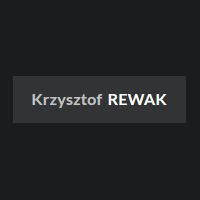
\includegraphics[width=.15\textwidth]{../_template/rewak.png}
		}
	\end{figure}

\end{frame}

\end{document}
